% Created 2022-09-24 Sat 23:50
% Intended LaTeX compiler: pdflatex
\documentclass[11pt]{article}
\usepackage[utf8]{inputenc}
\usepackage[T1]{fontenc}
\usepackage{graphicx}
\usepackage{longtable}
\usepackage{wrapfig}
\usepackage{rotating}
\usepackage[normalem]{ulem}
\usepackage{amsmath}
\usepackage{amssymb}
\usepackage{capt-of}
\usepackage{hyperref}
\graphicspath{{../../books/}}
% TIPS
% \substack{a\\b} for multiple lines text





% pdfplots will load xolor automatically without option
\usepackage[dvipsnames]{xcolor}

\usepackage{forest}
% two-line text in node by [two \\ lines]
% \begin{forest} qtree, [..] \end{forest}
\forestset{
  qtree/.style={
    baseline,
    for tree={
      parent anchor=south,
      child anchor=north,
      align=center,
      inner sep=1pt,
    }}}
%\usepackage{flexisym}
% load order of mathtools and mathabx, otherwise conflict overbrace

\usepackage{mathtools}
%\usepackage{fourier}
\usepackage{pgfplots}
\usepackage{amsthm, mathabx,  amsmath, commath}
\usepackage{amsfonts}

\usepackage{empheq}
\usepackage{tikz}
\usetikzlibrary{arrows.meta}
\usepackage[most]{tcolorbox}

\newtheorem{theorem}{Theorem}[section]
\newtheorem{definition}{Definition}[section]
\newtheorem{corollary}{Corollary}[section]
\newtheorem{example}{Example}[section]
\newtheorem{lemma}{Lemma}[section]
\newtheorem{proposition}{Proposition}[section]

\newcommand{\bl}[1] {\boldsymbol{#1}}
\newcommand{\Wt}[1] {\stackrel{\sim}{\smash{#1}\rule{0pt}{1.1ex}}}
\newcommand{\wt}[1] {\widetilde{#1}}


%For boxed texts in align, use Aboxed{}
%otherwise use boxed{}

\DeclareMathSymbol{\widehatsym}{\mathord}{largesymbols}{"62}
\newcommand\lowerwidehatsym{%
  \text{\smash{\raisebox{-1.3ex}{%
    $\widehatsym$}}}}
\newcommand\fixwidehat[1]{%
  \mathchoice
    {\accentset{\displaystyle\lowerwidehatsym}{#1}}
    {\accentset{\textstyle\lowerwidehatsym}{#1}}
    {\accentset{\scriptstyle\lowerwidehatsym}{#1}}
    {\accentset{\scriptscriptstyle\lowerwidehatsym}{#1}}
}

\usepackage{graphicx}
    
% text on arrow for xRightarrow
\makeatletter
%\newcommand{\xRightarrow}[2][]{\ext@arrow 0359\Rightarrowfill@{#1}{#2}}
\makeatother


\def \bx {\boldsymbol{x}}
\def \ba {\boldsymbol{a}}
\def \bI {\boldsymbol{I}}
\def \bt {\boldsymbol{t}}
\def \bb {\boldsymbol{b}}
\def \bA {\boldsymbol{A}}
\def \bX {\boldsymbol{X}}
\def \bu {\boldsymbol{u}}
\def \bS {\boldsymbol{S}}
\def \bZ {\boldsymbol{Z}}
\def \bz {\boldsymbol{z}}
\def \by {\boldsymbol{y}}
\def \bw {\boldsymbol{w}}
\def \bT {\boldsymbol{T}}
\def \bS {\boldsymbol{S}}
\def \bm {\boldsymbol{m}}
\def \bW {\boldsymbol{W}}
\def \bY {\boldsymbol{Y}}
\def \bH {\boldsymbol{H}}
\def \blambda {\boldsymbol{\lambda}}
\def \bPhi {\boldsymbol{\Phi}}
\def \btheta {\boldsymbol{\theta}}
\def \bmu {\boldsymbol{\mu}}
\def \bphi {\boldsymbol{\phi}}
\def \bSigma {\boldsymbol{\Sigma}}
\def \lb {\left\{}
\def \rb {\right\}}
\def \caln {\mathcal{N}}
\def \dissum {\displaystyle\Sigma}
\def \dispro {\displaystyle\prod}
\def \E {\mathbb{E}}
\def \Q {\mathbb{Q}}
\def \V {\mathbb{V}}
\def \R {\mathbb{R}}
\def \calq {\mathcal{Q}}
\def \calg {\mathcal{G}}
\def \caln {\mathcal{N}}
\def \calr {\mathcal{R}}
\def \calm {\mathcal{M}}
\def \calc {\mathcal{C}}
\def \bcup {\bigcup}

\makeindex
\usepackage{minted}
\author{wu}
\date{\today}
\title{6.824}
\hypersetup{
 pdfauthor={wu},
 pdftitle={6.824},
 pdfkeywords={},
 pdfsubject={},
 pdfcreator={Emacs 28.0.92 (Org mode 9.6)}, 
 pdflang={English}}
\begin{document}

\maketitle
\tableofcontents


\section{map reduce}
\label{sec:orgf7a5902}

\subsection{programming model}
\label{sec:orgcd26db0}
the computation takes a set of \textbf{input} key/value pairs, and produces a set of \textbf{output} key/value
pairs. The user of the MapReduce library expresses the computation as two functions: \textbf{Map} and
\textbf{Reduce}

\textbf{Map}, written by the user, takes an input pair and produces a set of \textbf{intermediate} key/value
pairs. The MapReduce library groups together all intermediate values associated with the same
intermediate key \(I\) and passes them to the \textbf{Reduce} function

The \textbf{Reduce} function, also written by the user, accepts an intermediate key \(I\)  and a set of
values for that key. It merges together these values to form a possibly smaller set of values.
Typically just zero or one output value is produced per Reduce invocation.

\subsubsection{example}
\label{sec:orga84ad4f}
\begin{minted}[]{python}
map(String key, String value):
  // key: document name
  // value: document contents
  for each word w in value:
    EmitIntermediate(w, "1")

reduce(String key, Iterator values):
  // key: a word
  // values: a list of counts
  int result = 0;
  for each v in values:
    results += ParseInt(v)
  Emit(AsString(result))
\end{minted}
The \texttt{map} function emits each word plus an associated count of occurrences. The \texttt{reduce} function
sums together all counts emitted for a particular word

\subsubsection{Types}
\label{sec:org4f2e030}
\begin{alignat*}{3}
&\text{map}&&\texttt{(k1,v1)}&&\to\texttt{list(k2,v2)}\\
&\text{reduce}\quad&&\texttt{(k2,list(v2))}&&\to\texttt{list(v2)}\\
\end{alignat*}

\subsubsection{More examples}
\label{sec:org2a3c35b}
\textbf{Distributed Grep}: the map function emits a line if it matches a supplied pattern. The reduce
function is an identity function that just copies the supplied intermediate data to the output

\textbf{Count of URL Access Frequency}: the map function processes logs of web page requests an outputs
\(\la\texttt{URL,1}\ra\). The reduce function adds together all values for the same URL and emits
a \(\la\texttt{URL,total count}\ra\) pair

\textbf{Term-vector per Host}: A term vector summarizes the most important words that occur in a document
 or a set of documents as a list of \(\la word,frequency\ra\) pairs. The map function emits a
 \(\la\texttt{hostname,term vector}\ra\) pair for each input document. The reduce function is passed
 all per-document term vectors for a given host. It add these term vectors together, throwing
 away infrequent terms, and then emits a final \(\la\texttt{hostname,term vector}\ra\) pair

\subsection{Implementation}
\label{sec:orgcfc9083}
\subsubsection{Execution Overview}
\label{sec:orgf67c1c6}
The \emph{Map} invocations are distributed across multiple machines by automatically partitioning the
input data into a set of \(M\) \emph{splits}. The input splits can be processed in parallel by
different machines. \emph{Reduce} invocations are distributed by partitioning the intermediate key
space into \(R\) pieces using a partitioning function (e.g., \(hash(key)\mod R\)). The number of
partitions and the partitioning function are specified by the user

\begin{figure}[htbp]
\centering
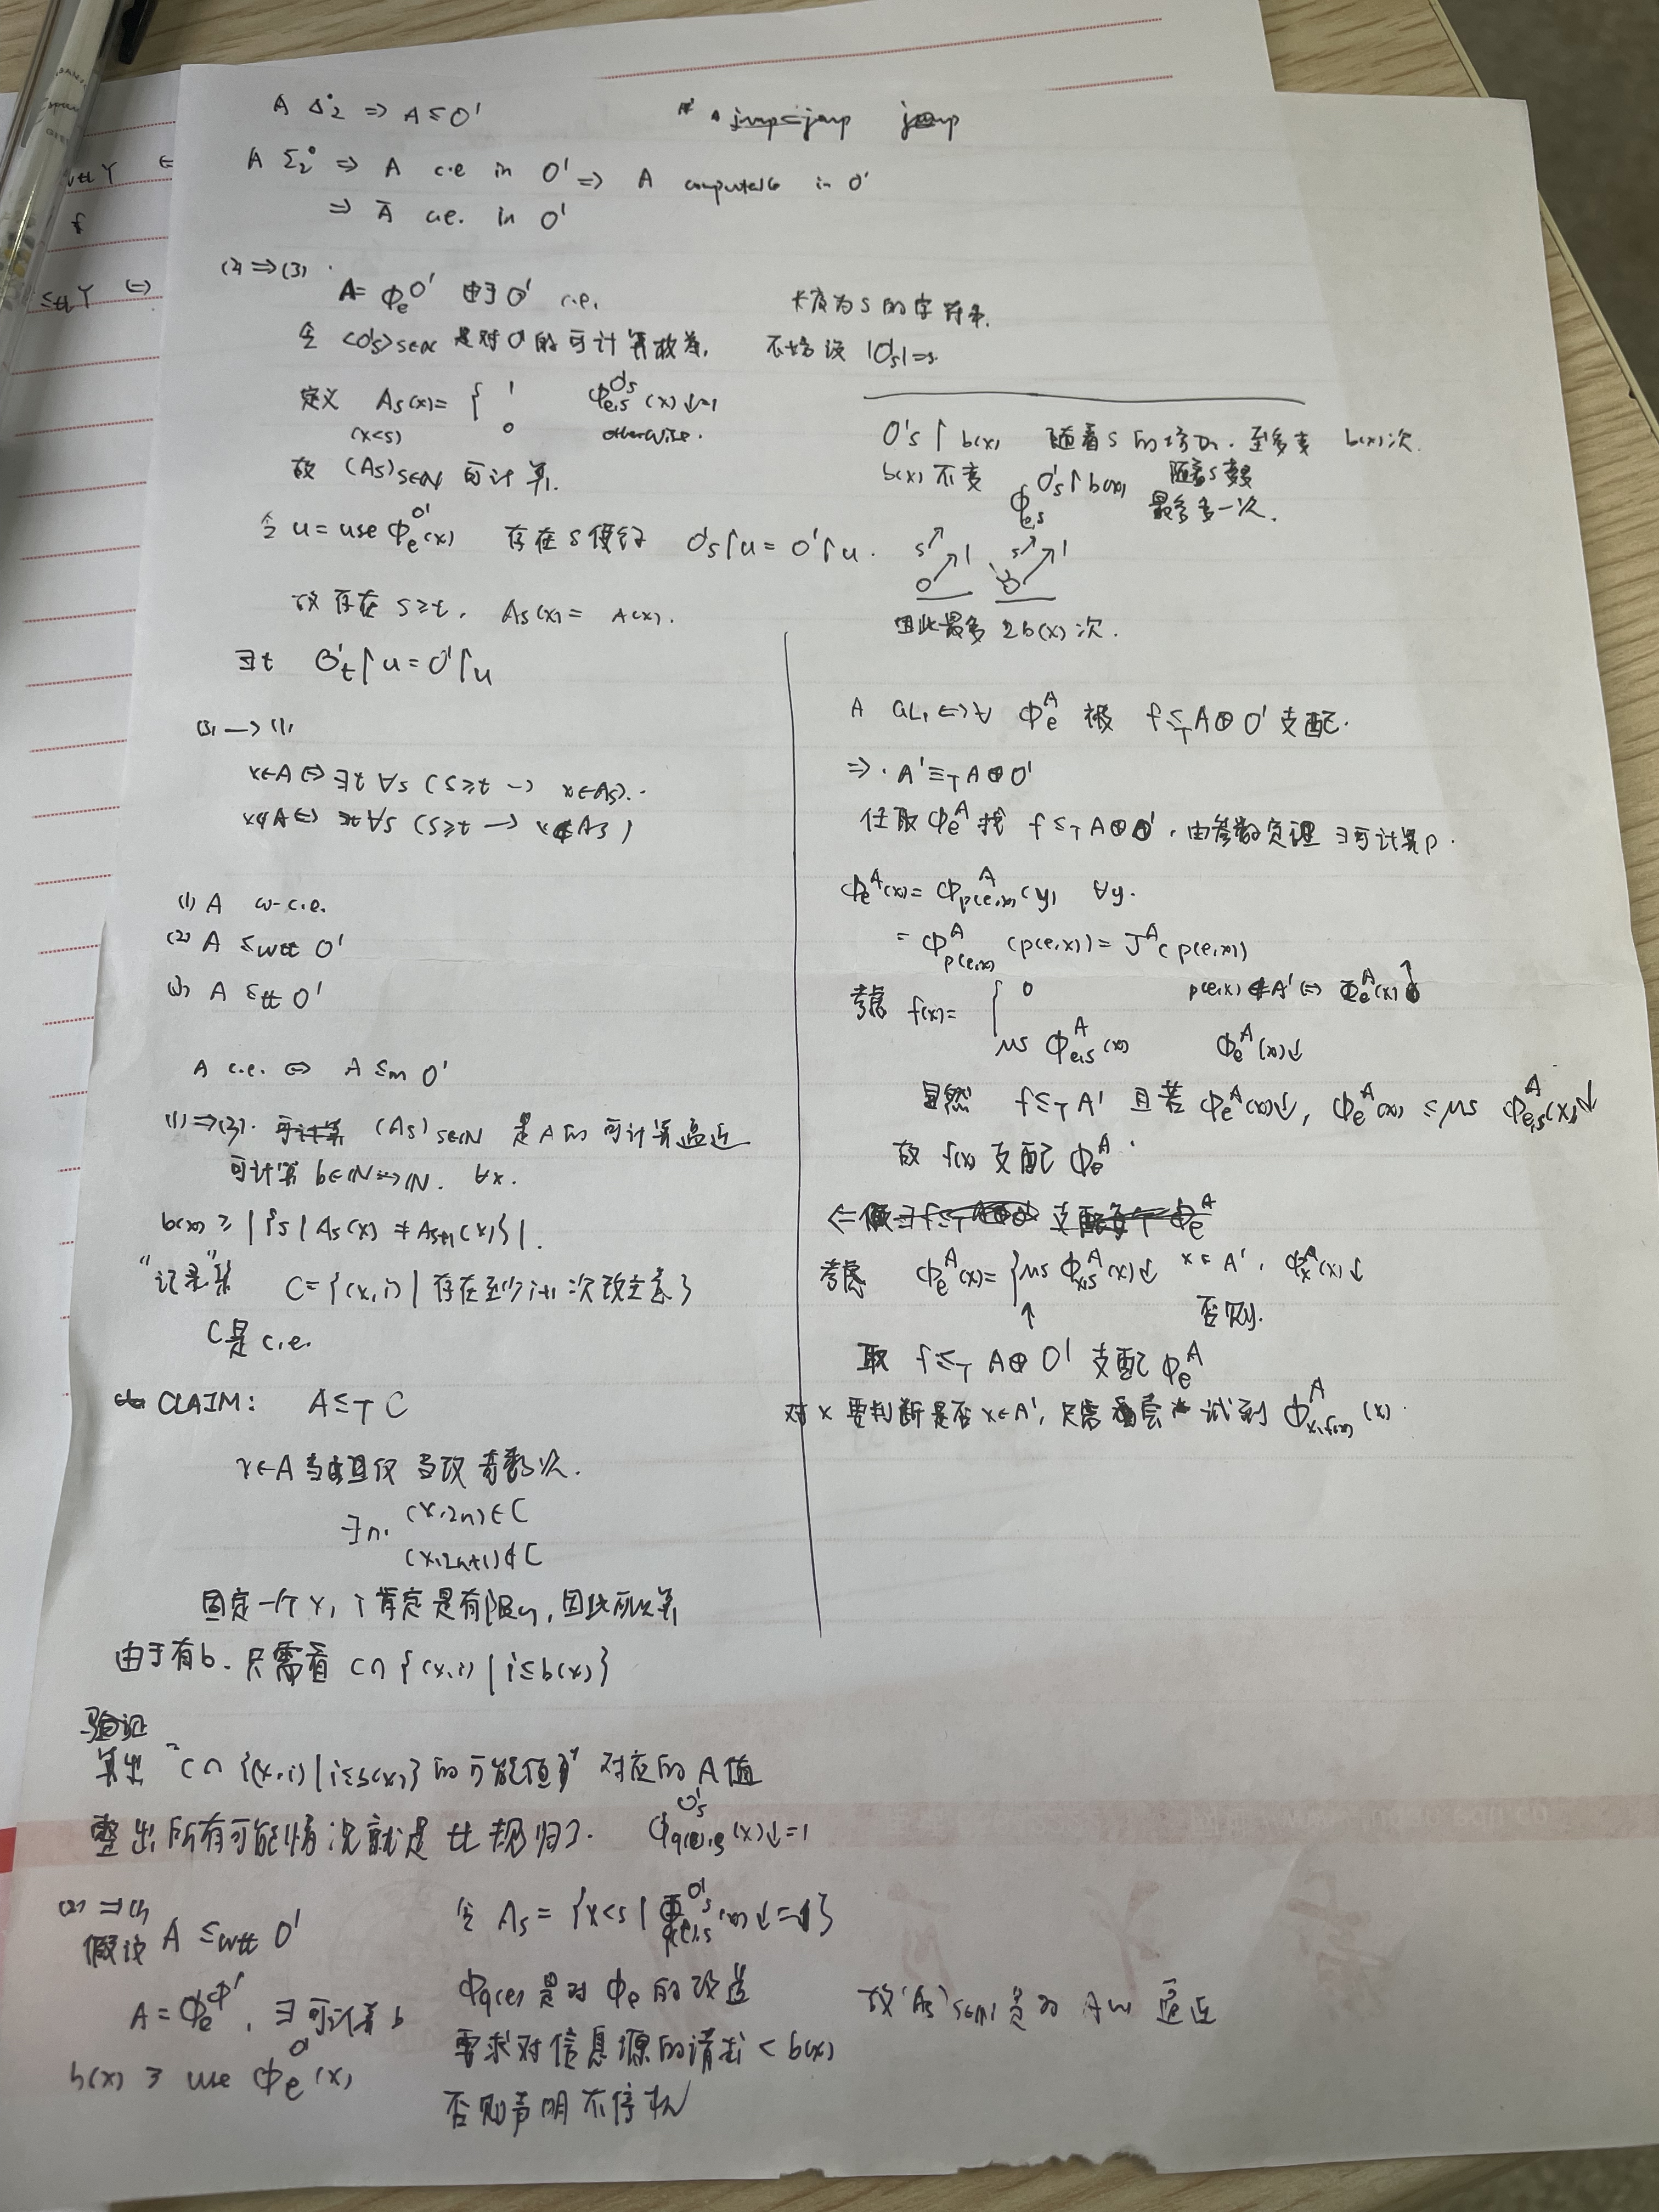
\includegraphics[width=\textwidth]{../images/6.824/1.png}
\label{}
\end{figure}

When the user program calls the \texttt{MapReduce} function, the following sequence of actions occurs
\begin{enumerate}
\item the MapReduce library in the user program first splits the input files into \(M\) pieces and
starts up many copies of the program on a cluster of machines
\item one of the copies of the program is special - the master. The rest are workers that are
assigned work by the master. there are \(M\) map tasks and \(R\) reduce tasks to assign. The
master picks idle workers and assigns each one a map task or a reduce task
\item a worker who is assigned a map task reads the contents of the corresponding input split. It
parses key/value pairs out of the input data and passes each pair to the user-defined \emph{Map}
function. The intermediate key/value pairs produced by the \emph{Map} function are buffered in memory
\item periodically, the buffered pairs are written to local disk, partitioned into \(R\) regions by
the partitioning function. The locations of these buffered pairs on the local disk are passed
back to the master, who is responsible for forwarding these locations to the reduce workers
\item when a reduce worker is notified by the master about these locations, it uses remote
procedure calls to read the buffered data from the local disks of the map workers. When a
reduce worker has read all intermediate data, it \textbf{sorts} it by the intermediate keys so that
all occurrences of the same key are grouped together. The sorting is needed because typically
many different keys map to the same reduce task. If the amount of intermediate data is too
large to fit in memory, an external sort is used
\item the reduce worker iterates over the sorted intermediate data and for each unique intermediate
key encountered, it passes the key and the corresponding set of intermediate values to the
user's \emph{Reduce} function. The output of the \emph{Reduce} function is appended to a final output file
for this reduce partition
\item when all map tasks and reduce tasks have been completed, the master wakes up the user
program. At this point, the \emph{MapReduce} call in the user program returns back the user code
\end{enumerate}
\subsubsection{Master data structures}
\label{sec:orgd81ecd3}
for each map task and reduce task, it stores the state (\emph{idle}, \emph{in-progress}, or \emph{completed}),
identity of the worker machine.

For each completed map task, the master stores the locations and sizes of the \(R\) intermediate
file regions produced by the map task. Updates to this location and size information are
received as map tasks are completed
\subsubsection{Fault tolerance}
\label{sec:orgf25206e}
\begin{enumerate}
\item worker failure
\label{sec:org69d6b84}
The master pings every worker periodically. If no response is received from a worker in a
certain amount of time, the master marks the worker as failed.

Completed map tasks are re-executed on a failure because their output is stored on the local
disk(s) of the failed machine and is therefore inaccessible
\item master failure
\label{sec:org5ddf01c}
It is easy to make the master write periodic checkpoints of the master data structures described
above.
\item Semantics in the presence of failures
\label{sec:org2ee61bb}
\end{enumerate}
\section{Raft paper}
\label{sec:orgebd48a6}
Raft is a consensus algorithm for managing a replicated log.
\subsection{Introduction}
\label{sec:orgaedfc3e}
Consensus algorithms allow a collection of machines to work as a coherent group that can survive
the failures of some of its members
\subsection{Replicated state machines}
\label{sec:org46444f3}
Replicated state machines are typically implemented using a replicated log, as shown in figure
\begin{figure}[htbp]
\centering
\includegraphics[width=.7\textwidth]{../images/6.824/2.png}
\label{}
\end{figure}
Each server stores a log containing a series of commands, which its state machine executes in
order. Each log contains the same commands in the same order, so each state machine processes
the same sequence of commands. Since the state machines are deterministic, each computes the
same state and the same sequence of outputs. Once commands are properly replicated, each
server’s state machine processes them in log order, and the outputs are returned to clients.

Consensus algorithms for practical systems typically have the following properties:
\begin{itemize}
\item they ensure \textbf{safety} (never returning an incorrect result) under all non-Byzantine conditions,
including network delays, partitions, and packet loss, duplication, and reordering
\item they are fully functional as long as any majority of the servers are operational and can
communicate with each other and with clients. Thus a typical cluster of five servers can
tolerate the failure of any two servers
\item they do not depend on timing to ensure the consistency of the logs
\item in the common case, a command can complete as soon as a majority of the cluster has responded
to a single round of remote procedure calls
\end{itemize}
\subsection{The Raft consensus algorithm}
\label{sec:orgc247361}
\href{https://eli.thegreenplace.net/2020/implementing-raft-part-3-persistence-and-optimizations/}{link}

\begin{figure}[htbp]
\centering
\includegraphics[width=.9\linewidth]{../images/6.824/3.pdf}
\label{}
\end{figure}


Raft implements consensus by first electing a distinguished \textbf{leader}, then giving the leader
complete responsibility for managing the replicated log. The leader accepts log entries from
clients, replicates them on other servers, and tell servers when it is safe to apply log entries
to their state machines.

Given the leader approach, Raft decomposes the consensus problem into three relatively
independent subproblems:
\begin{itemize}
\item \textbf{leader election}
\item \textbf{log replication}
\item \textbf{safty} : the key safety property for Raft is the State Machine Safety Property: if any server
has applied a particular log entry to its state machine, then no other server may apply a
different command for the same log index
\begin{itemize}
\item \textbf{Election Safety}: at most one leader can be elected
\item \textbf{Leader Append-Only}: a leader never overwrites or deletes entries in its log; it only append
new entries
\item \textbf{Log Matching}: if two logs contain an entry with the same index and term, then logs are
identical in all entries up through the given index
\item \textbf{Leader Completeness}: if a log entry is commited in a given term, then that entry will be
present in the logs of the leaders for all higher-numbered terms
\item \textbf{State Machine Safety}: if a server has applied a log entry at a given index to its state
machine, no other server will ever apply a different log entry for the same index
\end{itemize}
\end{itemize}
\subsubsection{Raft basics}
\label{sec:org8457912}
At any given time each server is in one of three states: \textbf{leader}, \textbf{follower} or \textbf{candidate}. In
normal operation there is exactly one leader and all of the other servers are followers.
\begin{itemize}
\item Followers are passive: they issue no requests on their own but simply respond to requests from
leaders and candidates.
\item The leader handles all client requests (if a client contacts a follower, the follower
redirects it to the leader)
\item Candidate is used to elect a new leader
\end{itemize}
\begin{figure}[htbp]
\centering
\includegraphics[width=.7\textwidth]{../images/6.824/4.png}
\label{}
\end{figure}

Raft divides time into \textbf{terms} of arbitrary length:
\begin{figure}[htbp]
\centering
\includegraphics[width=.7\textwidth]{../images/6.824/5.png}
\label{}
\end{figure}
Terms are numbered with consecutive integers. Each term begins with an \textbf{election}, in which one or
more candidates attempt to become leader. If a candidate wins the election, then it serves as
leader for the rest of the term. In some situations an election will result in a split vote, in
this case the term will end with no leader; a new term (with a new election) will begin shortly.
Raft ensures that there is at most one leader in a given term

Different severs may observe the transitions between terms at different times, and in some
situations a server may not observe an election or even entire terms. Terms act as a logical
clock in Raft, and they allow servers to detect obsolete information such as stable leaders.

Each server stores a \textbf{current term} number, which increases monotonically over time. Current terms
are exchanged whenever servers communicate; if one server's current term is smaller than the
other's, then it updates its current term to the larger value. If a candidate or leader
discovers that its term is out of data, it immediately reverts to follower state. If a server
receives a request with a stale term number, it rejects the request.

Raft servers communicate using remote procedure calls(RPCs), and the basic consensus algorithm
requires only two types of RPCs. RequestVote RPCs are initiated by candidates during elections,
and AppendEntries RPCs are initiated by leaders to replicate log entries and to provide a form
of heartbeat
\subsubsection{Leader Election}
\label{sec:orgacd9155}
Raft uses a heartbeat mechanism to trigger leader election.

When servers start up, they begin as followers. A server remains in follower state as long as it
receives valid RPCs from a leader or candidate. Leaders send periodic heartbeats (AppendEntries
RPCs that carry no log entries) to all followers in order to maintain their authority. If a
follower receives no communication over a period of time called the \textbf{election timeout}, then it
assumes there is no viable leader and begins an election to choose a new leader

To begin an election, a follower increments its current term and transitions to candidate state.
It then votes for itself and issues RequestVote RPCs \textbf{in parallel} to each of the other servers in
the cluster. A candidate continues in this state until one of three things happens:
\begin{enumerate}
\item it wins the election
\item another server establishes itself as leader
\item a period of time goes by with no winner
\end{enumerate}

A candidate wins an election if it receives votes from a majority of the servers in the full
cluster for the same term. Each server will vote for at most one candidate in a given term, on a
first-come-first-served basis (5.4 adds an additional restriction on votes). The majority rules
ensures that at most one candidate can win the election for a particular term (the \textbf{Election}
\textbf{Safe Property}) Once a candidate wins the election, it becomes leader. It then sends heartbeat
messages to all of the other servers to establish its authority and prevent new elections

While waiting for votes, a candidate may receive an AppendEntries RPC from another server claiming
to be leader. If the leader's term is at least as large as the candidate's current term, then
the candidate recognizes the leader as legitimate and returns to follower state. If the term in
the RPC is smaller than the candidate's current term, then the candidate rejects the RPC and
continues in candidate state.

The third possible outcome is that a candidate neither wins nor loses the election: if many
followers become candidates at the same time, votes could be split so that no candidate obtains
a majority. When this happens, each candidate will time out and start a new election by
incrementing its term and initiating another round of RequestVote RPCs. However, without extra
measures split votes could repeat indefinitely.

Raft uses randomized election timeouts to ensure that split votes are rare and that they are
resolved quickly. To prevent split votes in the first place, election timeouts are chosen
randomly from a fixed interval (e.g., 150-300ms). This spreads out the servers so that in most
cases only a single server will time out; it wins the election and sends single server will time
out.

The same mechanism is used to handle split votes. Each candidate restarts its randomized
election timeout at the start of an election, and it waits for that timeout to elapse before
starting the next election;
\subsubsection{Log replication [15/15]}
\label{sec:orgc0d8fa9}

Check \href{https://stackoverflow.com/questions/46376293/what-is-lastapplied-and-matchindex-in-raft-protocol-for-volatile-state-in-server}{this} for some explanation.

Each client request contains a command to be executed by the replicated state machines.
\begin{enumerate}
\item{$\boxtimes$} The leader appends the command to its log as a new entry, then issues AppendEntries RPCs in
parallel to each of the other servers to replicate the entry.
\item{$\boxtimes$} When the entry has been safely replicated, the leader applies the entry to its state machine
and returns the result of that execution to the client.
\item{$\boxtimes$} If followers crash or run slowly, or if network packets are lost, the leader retries
AppendEntries RPCs indefinitely (even after it has responded to the client) until all
followers
\end{enumerate}
eventually store all log entries.

Los are organized as below
\begin{figure}[htbp]
\centering
\includegraphics[width=.7\textwidth]{../images/6.824/6.png}
\label{}
\end{figure}
Each log entry stores a state machine command along with the term number when the entry was
received by the leader. The term numbers in log entries are used to detect inconsistencies
between logs and to ensure some of the properties. Each log entry also has an integer index
identifying its position in the log

The leader decides when it is safe to apply a log entry to the state machines; such an entry is
called \textbf{committed}.
\begin{itemize}
\item[{$\boxtimes$}] A log entry is committed once the leader that created the entry has replicated it on a
majority of the servers. This also commits all preceding entries in the leader's log,
including entries created by previous leaders.
\item[{$\boxtimes$}] The leader keeps track of the highest index it knows to be committed, and it includes that
index in future AppendEntries RPCs (including heartbeats) so that the other servers eventually
find out.
\item[{$\boxtimes$}] Once a follower learns that a log entry is committed, it applies the entry to its local state machine
\end{itemize}

Raft maintains the following properties, which together constitute the Log Machine Property:
\begin{itemize}
\item If two entries in different logs have the same index and term, then they store the same command
\item If two entries in different logs have the same index and term, then the logs are identical in
all preceding entries
\end{itemize}

The first property follows from the fact that a leader creates at most one entry with a given
log index in a given term, and log entries never change their position in the log.

The second property is guaranteed by a simple consistency check performed by AppendEntries.
\begin{enumerate}
\item{$\boxtimes$} When sending an AppendEntries RPC, the leader includes the index and the term in its log that
immediately precedes the new entries.
\item{$\boxtimes$} If the follower does not find an entry in its log with the same index and term, then it
refuses the new entries
\end{enumerate}
The consistency check acts as an induction

During normal operation, the logs of the leader and followers stay consistent, so the
AppendEntries consistency check never fails.

However, leader crashes can leave the log inconsistent,
\begin{figure}[htbp]
\centering
\includegraphics[width=.7\textwidth]{../images/6.824/7.png}
\label{}
\end{figure}

In Raft, the leader handles inconsistencies by forcing the follower' log to duplicate its own.
This means that conflicting entries in follower logs will be overwritten with entries from the
leader's log

To bring a follower's log into consistency with its own, the leader must
\begin{enumerate}
\item{$\boxtimes$} find the latest log entry where the two logs agree
\item{$\boxtimes$} delete any entries in the follower's log after that point
\item{$\boxtimes$} send the follower all of the leader's entries after that point
\end{enumerate}
All of these actions happen in response to the consistency check performed by AppendEntries
RPCs.

The leader maintains a \texttt{nextIndex} for each follower, which is the index of the next log entry the
leader will send to that follower
\begin{enumerate}
\item{$\boxtimes$} When a leader first comes to power, it initializes all \texttt{nextIndex} values to the index just
after the last one in its log (11 in figure)
\item{$\boxtimes$} If a follower's log is inconsistent with the leader's, the AppendEntries consistency check
will fail in the next AppendEntries RPC.
\item{$\boxtimes$} After a rejection, the leader decrements \texttt{nextIndex} and retries the AppendEntries RPC.
Eventually \texttt{nextIndex} will reach a point where the leader and follower logs match.
\item{$\boxtimes$} When this happens, AppendEntries will succeed, which removes any conflicting entries in the
follower's log and appends entries from the leader's log.
\end{enumerate}

Once AppendEntries succeeds, the follower's log is consistent with the leader's, and it will
remain that way for the rest of the term

If desired, the protocol can be optimized to reduce the number of rejected AppendEntries RPCs.
\begin{itemize}
\item When rejecting an AppendEntries request, the follower can include the term of the conflicting
entry and the first index it stores for that term. With this information, the leader can
decrement \texttt{nextIndex} to bypass all of the conflicting entries in that term
\item One AppendEntries RPC will be required for each term with conflicting entries, rather than one
RPC per entry
\end{itemize}
\subsection{Safety}
\label{sec:org3b2607c}
\subsubsection{election restriction}
\label{sec:org0503ce8}
Raft uses the voting process to prevent a candidate from winning an election unless its log
contains all committed entries.

A candidate must contact a majority of the cluster in order to be elected, which means that
every committed entry must be present in at least one of those servers. If the candidate's log
is at least as up-to-date as any other log in that majority, then it will hold all the committed
entries.

The RequestVote RPC implements this restriction: the RPC includes information about candidate's
log, and the voter denies its vote if its own log is more up-to-date than that of the candidate

Raft determines which of two logs is more up-to-date by comparing the index and term of the last
entries in the logs.
\subsubsection{Committing entries from previous terms}
\label{sec:org8a60107}
\begin{itemize}
\item A leader knows that an entry from its current term is committed once that entry is stored on
a majority of the serves.
\item If a leader crashes before committing an entry, future leaders will attempt to finish
replicating the entry.
\item However, a leader cannot immediately conclude that an entry from a previous term is committed
once it is stored on a majority of servers
\end{itemize}

Below is an illustration:
\begin{figure}[htbp]
\centering
\includegraphics[width=.7\textwidth]{../images/6.824/8.png}
\label{}
\end{figure}

To eliminate problems like the one in figure, Raft never commits log entries from previous terms
by counting replicas. Once an entry from the current term has been committed, then all prior
entries are committed indirectly because of the Log Machting Property
\subsubsection{Safety argument}
\label{sec:org2b841d6}
We argue the Leader Completeness Property here (if a log entry is commited in a given term, then
that entry will be present in the logs of the leaders for all higher-numbered terms)

We assume that the Leader Completeness Property does not hold, then we prove a contradiction.

Suppose the leader for term T (leader\textsubscript{T}) commits a log entry from its term, but
that log entry is not stored by the leader of some future term. Consider the smallest term U>T
whose leader (leader\textsubscript{U}) does not store the entry
\end{document}
